\section{Marine Perception}
In the past few years, there has been a growing interest in datasets related to maritime activities. One of the first and most cited works in Marine Perception is VAIS by Zhang et al.\cite{Zhang_2015_CVPR_Workshops}, the first publicly available dataset of paired visible and infrared ship imagery. This dataset contains more than 1,000 paired RGB and infrared images among six ship categories - merchant, sailing, passenger, medium, tug, and small, and the ontology is compliant with COLREGs ie; the detections from a model developed with this ontology can be directly used in a COLREGs compliant ASV for path planning and other downstream autonomous operation tasks. The authors benchmarked their results using two off-the-shelf classifiers, a 16-layer CNN and a Gnostic Fields with SIFT features. Their work was influential in demonstrating the application of deep neural networks for marine perception tasks. The six proposed categories of ships are a good start. However, they can be further refined and improved by including stationary obstacles and reducing the number of powerboat classes to a single class, since COLREGs have no rules set according to the size of a vessel, but only its category. The dataset was also only collected from a single stationary point and not from a moving vessel, leading to a desire for dataset diversity for better-trained models. 
\\

The authors captured more than two terabytes of data in nine days. The data consisted of synchronized image sequences using a horizontal stereo rig, as shown in the figure below. The captured images were synchronized to retrieve one frame
per second from each camera by matching the two closest microsecond timestamps within each full second. Before data capture, the camera focus and exposure were manually adjusted to account for environmental conditions. Each time ships appeared, the authors captured an image and recorded it until the size of the ships became insignificant. During the day, the authors used a monocular and identified each ship’s name for later use during annotation. At night, the names of the ships were discovered using the MarineTraffic Android application, which shows the locations of nearby ships that relayed the information from the Automatic Identification System (AIS) in real time, but this was mostly limited to larger vessels that usually always equip AIS transponders as compared to smaller recreational consumer vessels. 
\begin{figure}[H]
    \centering
    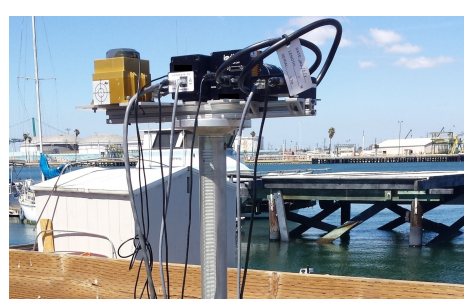
\includegraphics[width=\textwidth,height=5cm,keepaspectratio=true]{src/Images/vais_gear.PNG}
    \caption{
     The RGB-IR Camera setup developed by the VAIS team. \cite{Zhang_2015_CVPR_Workshops}
     }
\end{figure}
\\

For each unique ship in the dataset, the authors manually drew
bounding boxes in the images, labeled the
ship type, and assigned it the name recorded using the
monocular or AIS data. In case the ship’s name was absent, the authors assigned it a short description based on its appearance. Since the images were captured as image sequences at one frame per second, consecutive frames, which were near-duplicates, were removed, and bounding boxes with areas smaller than a reasonable threshold (200 pixels) were discarded from the dataset. The dataset consists of 2865 images (1623 visible and 1242 IR), of which there are 1088 corresponding pairs. There are a total of 154 nighttime IR images as well. The dataset includes 264 uniquely named ships in six "coarse-grained" categories or 15 "fine-grained". 
\\

The data set was then divided into train/test sets for benchmarking. This resulted in 539 image pairs and 334 singletons for training and 549 image pairs and 358 singletons for testing. All night images were assigned to testing. The authors trained a to observe model performance independently. The authors found the CNN to perform better overall; however, both the models struggled with nighttime data. This could be explained by the limited number of data samples for training, as well as fewer number of hidden layers, which leads to weaker classification capabilities. 
\begin{figure}[H]
    \centering
    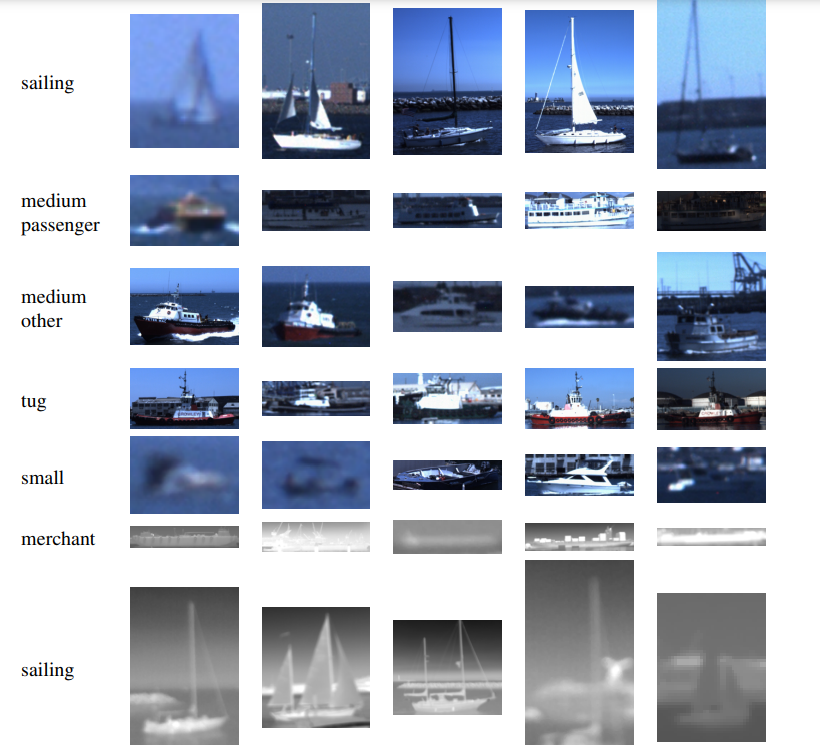
\includegraphics[width=\textwidth,height=10cm,keepaspectratio=true]{src/Images/vais_data.PNG}
    \caption{
     Sample of the VAIS Dataset. \cite{Zhang_2015_CVPR_Workshops}
     }
\end{figure}
\\

Another major inspiration and a source of collaboration was \cite{defilippo2021robowhaler}'s work on their Robowhaler project. Robowhaler (vessel name R/V Philos) was a Boston Whaler Outrage 350 donated by Mercury Marine, a part of Brunswick Corporation, as part of their collaboration efforts with the Sea Grant Laboratory for furthering research and interest in marine autonomy. The primary objectives of their work were to collect on-water datasets (which are currently publicly available) as well as test behaviors and algorithms for autonomous operations based on the Moos-IvP autonomy stack\cite{benjamin2009overview}. The vessel had a modified interface to the vessel's control systems thanks to work by Mercury Engineers. It was equipped with sensors for navigation like INS/GPS, sensing solutions like cameras (IR and RGB), Marine Radars, Lidar, and an on-vessel computer equipped with an Nvidia GPU. The autonomy software stack consisted of a combination of Ros one-MOOS/IVP, where Ros - Robot Operating System\cite{ros} one was used as the robotics middleware to interface with the sensors using either their native Ros drivers developed by the sensor manufacturer or self-developed by the Robowhaler team for their experimental purposes, and MOOS-IvP\cite{ivp_stack} was used for higher-level path planning or autonomous behavior planning. 
\\

Their work has been critical in the development of interest in the field of marine autonomy and in the advancement of collaboration between academia, the government, and industry for the research and development of autonomous maritime solutions. It was their work that gave me my start in the field of computer vision and marine autonomy. Their work also released one of the largest maritime datasets available publicly, and the authors contributed significantly towards the advancement of MOOS-IvP's software stack. Some of the challenges the paper did not provide a clear solution for such as hardening of the sensors to enable them to survive harsh maritime environments, and no suggested ontology or annotations for the RGB or IR images. The authors could also investigate memory-effective sensor data log formats such as MCAP or provide any solutions for real-time capture of sensor data such as images and GPS logs using on-board connectivity options\cite{benjamin2009overview}.
\begin{figure}[H]
    \centering
    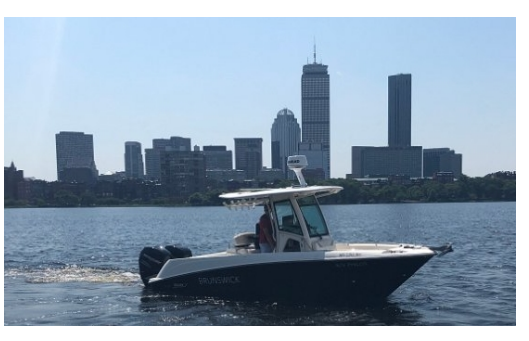
\includegraphics[width=\textwidth,height=10cm,keepaspectratio=true]{src/Images/philos.PNG}
    \caption{
     Philos cruising down Boston's Charles River.\cite{defilippo2021robowhaler}
     }
\end{figure}
\\

The authors developed two different perception stacks for different data collection seasons. For the 2020-2021 data collection missions, they chose the perception stack shown in the figure below. The cameras were mounted on an 80/20 bar that was welded to the vessel's hardtop, while the radar and lidar were mounted on top of the hardtop. The sensor suite included forward-facing IR and RGB cameras, providing approximately 145° horizontal field of view and 360° coverage from the marine radar and velodyne lidar. They chose a Simard 4G Broadband radar with 360-degree coverage that typically sends returns at 5-10Hz. They used FLIR Pointgrey cameras with 1280 x 1024 resolution and 48° horizontal FOV for the RBG camera, while the IR camera was a FLIR ADK infrared (IR) camera, with 640 x 512 resolution and 75° horizontal FOV. In total, the authors used two IR cameras, three RGB cameras, one radar, and one lidar. The navigation stack consisted of two INS modules, an SBG Systems Ellipse2-D Dual Antenna RTK INS, and a secondary MTi 670 GNSS/INS. Both sensors provide roll, pitch, yaw, heading, heave, velocity, and position\cite{benjamin2009overview}.
\begin{figure}[H]
    \centering
    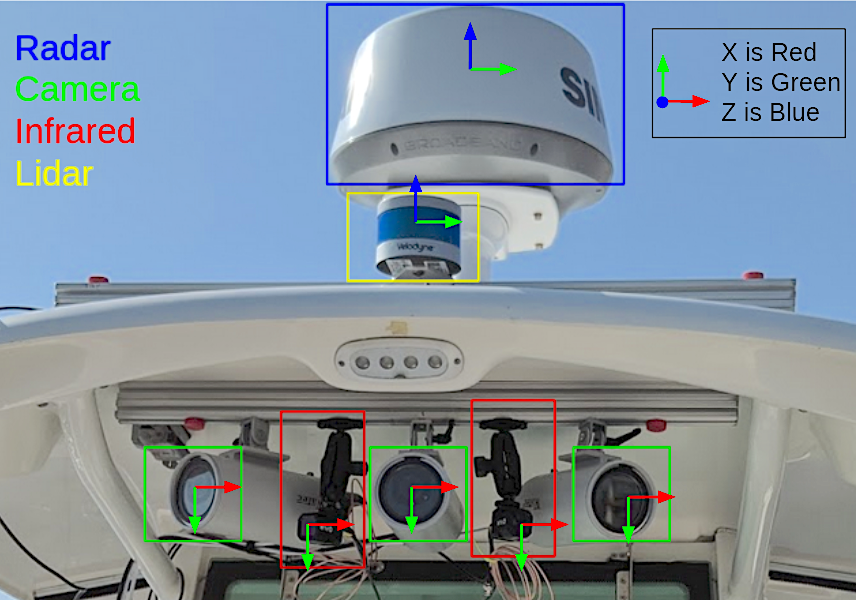
\includegraphics[width=\textwidth,height=6cm,keepaspectratio=true]{src/Images/philos_sensors.png}
    \caption{
     Philos sensor configuration\cite{defilippo2021robowhaler}.
     }
\end{figure}

\begin{figure}[H]
    \centering
    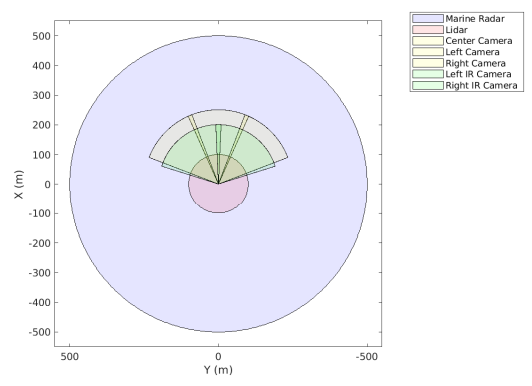
\includegraphics[width=\textwidth,height=6cm,keepaspectratio=true]{src/Images/philos_coverage.PNG}
    \caption{
     Philo's sensor coverage while equipped with the five cameras, radar, and lidar perception stack.  \cite{defilippo2021robowhaler}
     }
\end{figure}
\\

The figure below shows the autonomous software on board Philos. The authors based their software stack on the "Backseat control" architecture that divides the vessel's vehicle control ("front seat") and the vehicle autonomy software ("back seat"). The "front seat" is responsible for real-time vessel control, while the "back seat" is responsible for autonomous dynamic decision making and behavior planning. The main motivation behind this architecture was to develop autonomy software for ASV/AUV such that the autonomy solution chosen is independent of the dynamic control specifics of any given vehicle. This ensures the portability of software and the reuse of code. It also prevents any autonomy software developers from being tied to a particular vehicle manufacturer's autonomy software and support\cite{eickstedt2010backseat}. 
\begin{figure}[H]
    \centering
    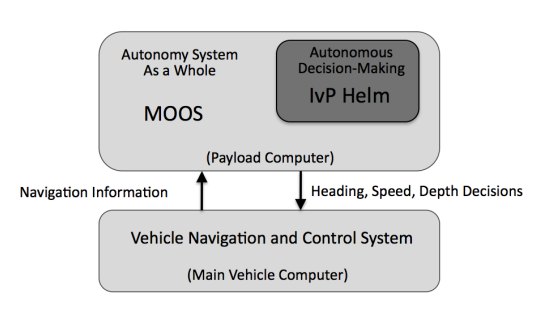
\includegraphics[width=\textwidth,height=8cm,keepaspectratio=true]{src/Images/backseat_arch.PNG}
    \caption{
     Philos Back seat architecture \cite{defilippo2021robowhaler}
     }
\end{figure}
\\

It also provides redundancy by separating the vehicle control from the decision-making system just in case any erroneous commands or behaviors were generated, or in case of any critical failure of the autonomy software, the vessel controls can still be enabled. In Philos, MOOS is the back seat; it commands the vessel's heading and speed by sending either velocity or heading update commands to the vessel control system, i.e. the front seat, using the MOOS-CAN interface. The vessel's control system issues commands to the engines and returns any state change information, such as navigation and vehicle information, to the MOOS-CAN interface and the backseat. On top of this software architecture, the authors leveraged docker to provide a platform and middleware agnostic software library. The current setup consists of a Ros one system for interfacing with the sensors and performing sensing operations like radar return clustering for object detection, camera object detection/segmentation, etc. These results from the sensing phase are sent to MOOS-IvP via NMEA messages\cite{enwiki:1168017133}. Based on the inputs, the MOOS is able to react dynamically and make behavior decisions, which are then passed to the control system in the form of NMEA messages using the MOOS-CAN interface.\cite{benjamin2009overview}
\begin{figure}[H]
    \centering
    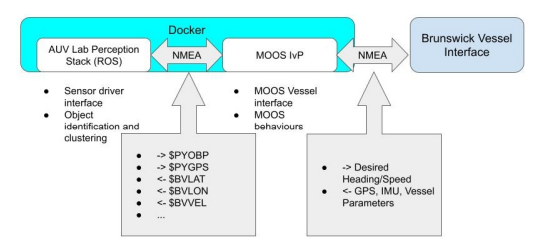
\includegraphics[width=\textwidth,height=8cm,keepaspectratio=true]{src/Images/philos_arch.PNG}
    \caption{
     Philos Autonomy software stack \cite{defilippo2021robowhaler}
     }
\end{figure}
\\

Philos was designed with modularity in mind. Along with easier sensor hardware mounting, the suite of perception sensors is interchangeable. It can range from a single camera to a full suite of various modalities of perception sensors, such as radar, lidar, camera, and IR. Each sensor is configured through environmental parameters via Docker launch scripts and can be swapped in and out quickly on the fly as required by the data collection mission or changing environmental conditions. Sensor fusion algorithms are designed to
cluster objects from the radar and lidar and report via NMEA
message strings to the MOOS obstacle manager. The obstacles are then used to provide the optimal direction and speed for the vessel to navigate safely through an obstacle field.\cite{benjamin2009overview}
\begin{figure}[H]
    \centering
    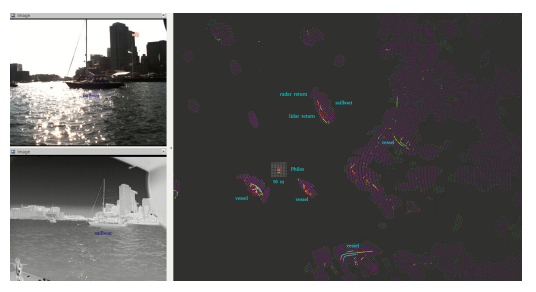
\includegraphics[width=\textwidth,height=8cm,keepaspectratio=true]{src/Images/philos_op.PNG}
    \caption{
     Philos data capture at a mooring field in Boston.  \cite{defilippo2021robowhaler}
     }
\end{figure}
\\

The author released a marine perception dataset that can be used by industry professionals and researchers to test algorithms related to the sensor modalities, such as camera object detection and radar point clustering. The dataset consists of raw, unprocessed data from all navigation and perception sensors, with minor issues such as occasional dropouts, glare from the sun, rain/snow on camera lenses, or sensor jitter from rough seas. The dataset also provides multiple vehicle path trajectories, some with loop closures, in various weather conditions and at different vessel speeds, which is useful for testing trajectory estimation algorithms.\cite{benjamin2009overview}
\\

The authors conducted autonomous behavior tests by focusing on the potential use of autonomous surface vessels (ASVs) in aquaculture to monitor nearshore and offshore fish farms autonomously. The authors developed some navigation and obstacle avoidance algorithms or MOOS behaviors, which they found to be crucial for operating an autonomous surface vessel within an aquaculture farm and during general transit. They imagined an aquaculture farm with multiple buoys and floating structures as an operational area through which the ASV must navigate with caution.\cite{benjamin2009overview}
\begin{figure}[H]
    \centering
    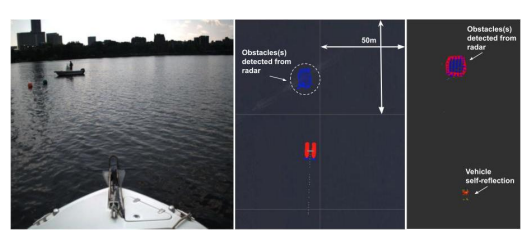
\includegraphics[width=\textwidth,height=10cm,keepaspectratio=true]{src/Images/philos_test.PNG}
    \caption{
     On the left, we can see the camera view from the center RGB camera, which shows us the buoys and the vessel in front of Philos. The center view is the MOOS-IvP birds-eye view of Philos along with the detected obstacles. On the right, RVIZ presents a bird's-eye view of clustered obstacles as a blue circle with a red perimeter.\cite{defilippo2021robowhaler}
    }
\end{figure}
\\

The authors reported promising results from preliminary tests for navigating Philos through an obstacle field. Philos detected obstacles and their approximate location, which were then passed on to the MOOS-IvP obstacle manager. The obstacles within the vessel's path were expanded on the basis of a user-defined buffer region, and the vessel safely avoided the obstacles by taking a new path around them within that region. The obstacle manager was able to correct for any new obstacles or changes in current obstacles and provide a safe path for each update. The tests were performed live on water on board Philos, and conducted on the Charles River, as shown in the figure above.\cite{defilippo2021robowhaler}
\\

Zust et al. \cite{Zust_2023_ICCV} published "LaRS: A Diverse Panoptic Maritime Obstacle Detection Dataset and Benchmark", is the first-ever benchmark for maritime panoptic obstacle detection. It features scenes from a wide range of water bodies, including lakes, rivers, and seas. LaRS is unique because it contains the largest diversity in locations, scene types, obstacle classes, and acquisition conditions compared to other related datasets. The dataset comprises more than 4000 per-pixel labeled keyframes, each with nine preceding frames to enable utilization of the temporal texture, which adds up to over 40k frames. Their work is pivotal in providing a one-of-a-kind dataset, and benchmark, however, is limited by the skewed distribution of objects (dataset consists of 90\% boat class object masks),  
\begin{figure}[H]
    \centering
    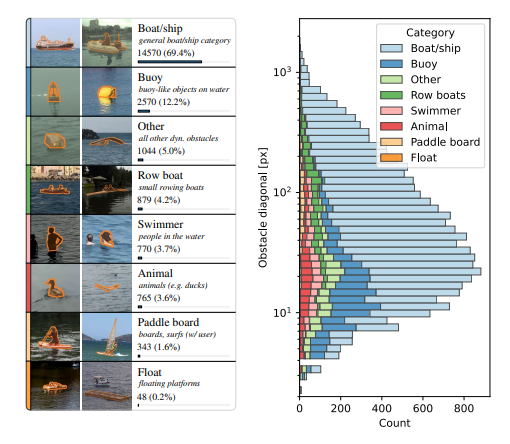
\includegraphics[width=\textwidth,height=5cm,keepaspectratio=true]{src/Images/lars_dist.PNG}
    \caption{
     Distribution of object classes in the LaRS dataset. \cite{Zust_2023_ICCV}
     }
\end{figure}
\\

Each keyframe is annotated with 8 thing/object classes (boat, row boat, paddle board, buoy, swimmer, animal, float, and other class), 3 stuff classes (shores and piers), and 19 global scene attributes relevant for navigation (like fog, wake, rough, day-like, sun glitter etc). Additionally, the authors report the results of 27 semantic and panoptic segmentation models, along with several performance insights. The authors sourced the dataset 1) from public online videos featuring various activities captured from boats around the world, 2) recorded new sequences in a number of different geographic locations themselves, and 3) included the most challenging scenes from existing maritime datasets. Their benchmark method is comprised of splitting the dataset into training (65\%), validation (5\%), and test (30\%) sets, and models are trained on the training set, with the validation set used for stopping criterion, and the performance is evaluated on the test set. The evaluation protocol included two tasks: 1) the classical semantic-segmentation-based obstacle detection and 2) panoptic-segmentation-based obstacle detection. 
\\

In total 19 models were evaluated such as maritime-specific obstacle detection models WaSR, WODIS, IntCatchAI and general semantic segmentation models such as FCN, UNet, DeepLabv3, DeepLabv3+, PointRend, KNet, three lightweight convolutional models BiSeNetv1, BiSeNetv2, STDC, two transformer-based models SegFormer, Segmenter and three temporal semantic segmentation models CSANet, TMANet and WaSRT. MMSegmentation was used for training and evaluation code except for a few models which provided their own training and evaluation code. The models were trained on 2x
NVIDIA V100 GPUs with a batch size of 8. Runtimes were
estimated in frames per second (FPS) on a single GPU. 
\begin{figure}[H]
    \centering
    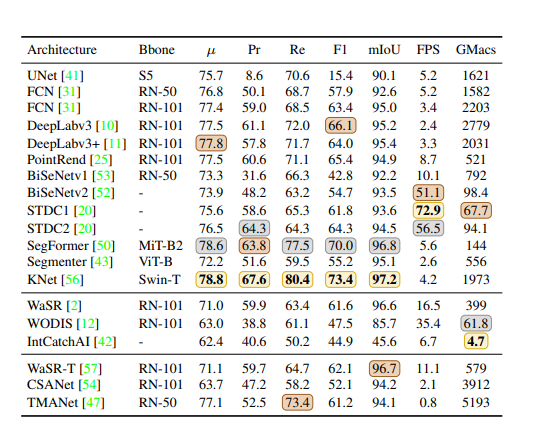
\includegraphics[width=\textwidth,height=7cm,keepaspectratio=true]{src/Images/lars.PNG}
    \caption{
     Lars Benchmarks\cite{Zust_2023_ICCV}
     }
\end{figure}
\\

The authors found that KNet achieved the best overall results,
followed by SegFormer.  These models also had the highest F1 indicating very good obstacle detection performance (good precision and recall). These models were also found to perform better than other models with respect to detecting small objects like buoys, people's faces etc. From their findings, we can see how Transformer-based approaches have proved their effectiveness in the maritime domain as well. However, transformer based models didn't have the best FPS performance which could result in slower adoption due to the additional GPU compute required to run these models in a realtime or close to realtime setting required for real world application. The temporal based models didn't outperform the single-frame approaches despite the additional input context. With respect to the panoptic segmentation task, particularly panoptic quality, PQ, performance, Swin-B-based Mask2Former was the best performer, followed by Panoptic FPN, and Swin-T-based Mask2Former. 
\begin{figure}[H]
    \centering
    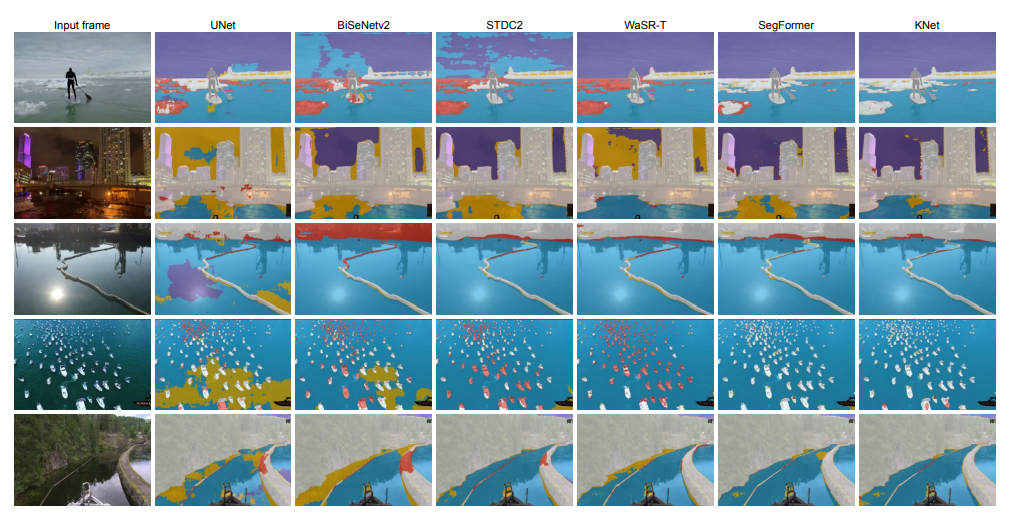
\includegraphics[width=\textwidth,height=7cm,keepaspectratio=true]{src/Images/lars_op.PNG}
    \caption{
     Qualitative semantic segmentation results from the benchmark\cite{Zust_2023_ICCV}
     }
\end{figure}

\begin{figure}[H]
    \centering
    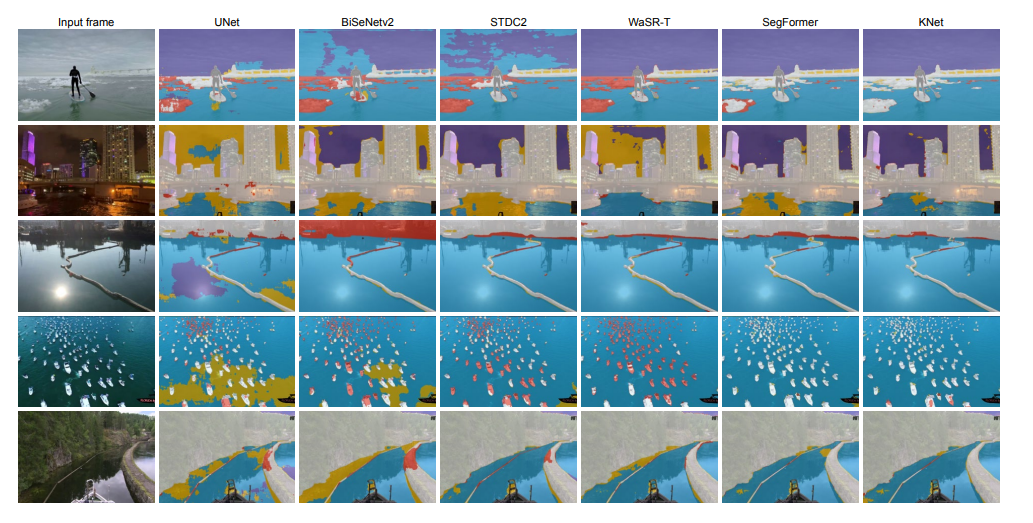
\includegraphics[width=\textwidth,height=7cm,keepaspectratio=true]{src/Images/lars_op_2.PNG}
    \caption{
     Qualitative panoptic segmentation results from the benchmark\cite{Zust_2023_ICCV}
     }
\end{figure}
\\

Another publicly available large-scale marine perception dataset released is MARVEL published by Gundogdu et al.\cite{gundogdu2017marvel}. The inspiration behind their work was to develop a state-of-the-art dataset for Visual classification of maritime vessels for the naval security and surveillance domain. MARVEL consists of over 2 million user-uploaded images organized using information from publicly available websites. The images were categorized into 109 classes of vessels based on image attributes such as vessel identity, type, etc. Furthermore, 26 superclasses were developed by combining heavily populated classes with a semi-automatic clustering scheme. For the evaluation of the dataset, the authors conducted experiments with useful maritime applications such as vessel classification, verification, retrieval, and recognition\cite{gundogdu2017marvel}. Modern day computer vision approaches require a lot of data with good dataset diversity. The author's efforts directly contributes towards this effort. However, their dataset is not compilant with classes required by COLREGs. It does not have any annotations like bounding boxes, which could lead to significant rework for anyone trying to adopt this dataset for application in a COLREGs compliant ASV. 
\begin{figure}[H]
    \centering
    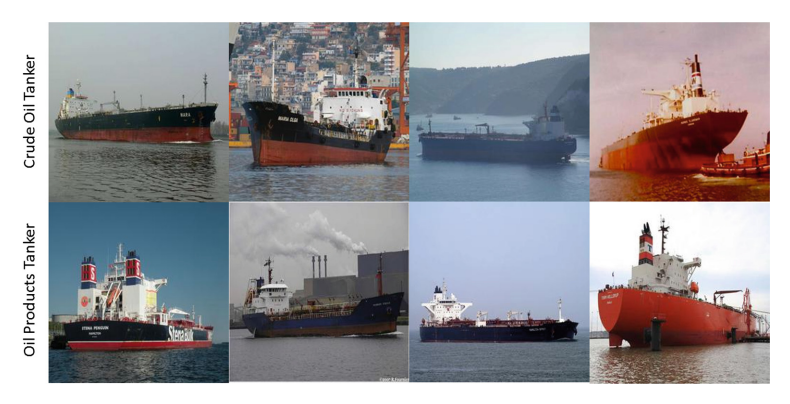
\includegraphics[width=\textwidth,height=7cm,keepaspectratio=true]{src/Images/marvel_sample.PNG}
    \caption{
     Vessel category example from MARVEL\cite{gundogdu2017marvel}
     }
\end{figure}
\\

The primary source of data was the website "Shipspotting.com"\cite{ship_website}. The authors collected more than 2 million images from this website, where hobby photographers upload images of maritime vessels with various descriptors, including vessel types, photo categories, gross tonnage, draft, built year, International Maritime Organization (IMO) number, and more. The dataset was organized based on vessel attributes such as beam, build year, draft, flag, gross tonnage, IMO number, vessel name, length, and vessel type. The most descriptive and visually meaningful features were found to be the type of vessel, photo category, and IMO number. Vessel type was assigned based on the type of cargo the vessel would transport, such as passenger ships, container ships, etc. The dataset includes 1,607,190 images with annotated vessel types belonging to one of 197 categories. The photo category provided visual descriptions of the vessel, such as the production period of a container ship. All the collected images were assigned a photo category out of the 185 categories. The third category was the IMO number, which is an identification number that uniquely identifies registered ships in the IMO database. More than 1,628,056 of the collected images are annotated with IMO numbers, and the dataset contains more than 103,701 unique IMO numbers.
\begin{figure}[H]
    \centering
    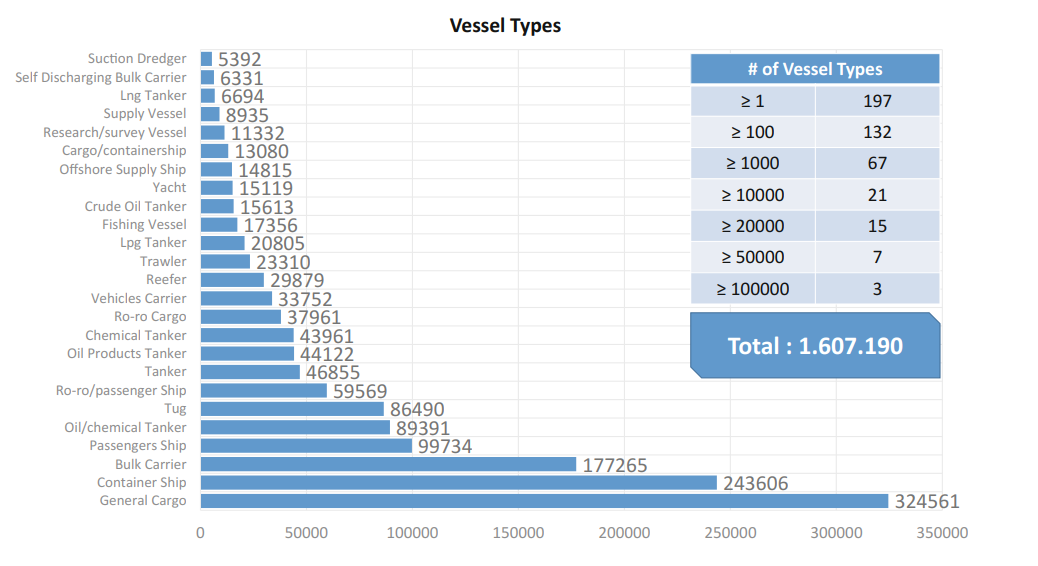
\includegraphics[width=\textwidth,height=7cm,keepaspectratio=true]{src/Images/marvel_types.PNG}
    \caption{
     Distribution of Vessel Types in MARVEL\cite{gundogdu2017marvel}
     }
\end{figure}
\\

To evaluate MARVEL, the authors introduced the maritime application - (1) vessel classification which would classify a vessel into its vessel type, based on the content of the cargo that the ship carried, (2) vessel verification, which identified if any two vessel images were of the same unique vessel, i.e., if both the vessels had the same IMO (3) vessel retrieval, i.e., image-based similarity search, and (4) vessel recognition for establishing if two vessels fall under the same vessel or photo type. For vessel classification, a set of superclasses was developed since some vessel types could overlap. It may contain more than one vessel category and for scenarios where the cargo would not be visible.
\begin{figure}[H]
    \centering
    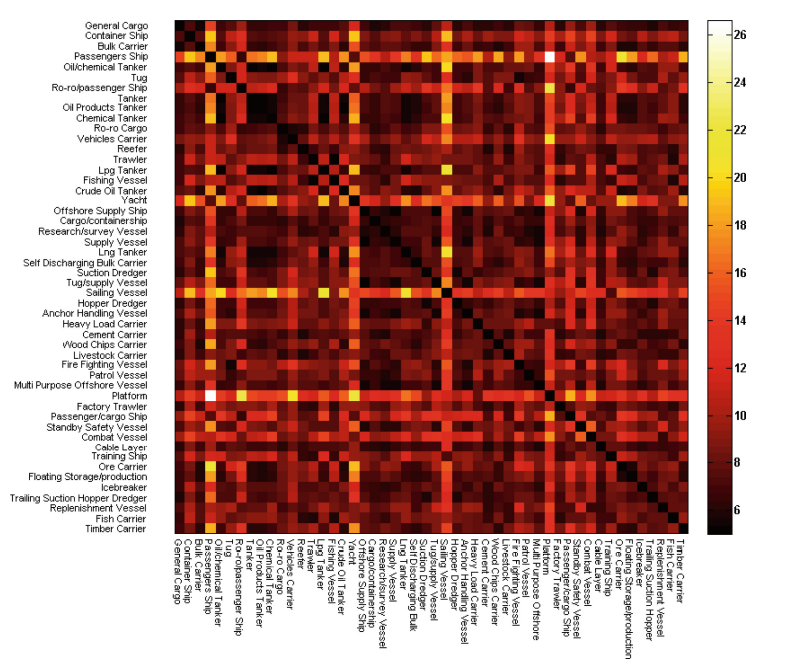
\includegraphics[width=\textwidth,height=10cm,keepaspectratio=true]{src/Images/marvel_diss_matrix.PNG}
    \caption{
     Dissimilarity matrix of the 50 vessel type superclasses\cite{gundogdu2017marvel}. 
     }
\end{figure}
\\

The authors used the first 50 vessel types that had the most examples and sorted them according to their quantity. They used the vessel type with the largest number of examples to generate superclasses. To analyze the similarities between the vessel types, they used a pre-trained convolutional neural network to extract the image's vector embedding representation and used the symmetrized divergence as the dissimilarity index. Then they calculated a dissimilarity matrix for the 50 selected vessel types. The authors then utilized the calculated dissimilarity matrix to develop a further grouping of classes. If the dissimilarity index of a pair of classes is below a threshold, the pair is assigned to the same superclass. The threshold is increased until a point where semantically irrelevant classes (human supervision is adopted here) start to merge and is defined as the final threshold for clustering. This process finally resulted in 26 superclasses. 
\begin{figure}[H]
    \centering
    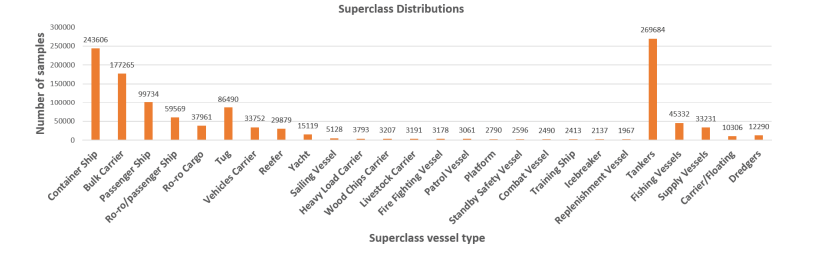
\includegraphics[width=\textwidth,height=10cm,keepaspectratio=true]{src/Images/marvel_superclasses.PNG}
    \caption{
     Distribution of MARVEL's 26 Superclasses\cite{gundogdu2017marvel}. 
     }
\end{figure}
\\

For Superclass Classification task, the authors trained a deep CNN architecture called AlexNet, using the default and recommended parameters without batch normalization. To avoid the imbalance between the superclasses, the authors only selected equal numbers of samples per class for both training and testing. For the superclasses with examples less than the required quantity of training samples, the authors utilized popular dataset augmentation methods to generate additional data. The training and test sets finally contained 212,992 and 26,624 examples respectively with 140K unique examples. The
classification task performance was measured by the help of the normalized confusion matrix. The final performance measure is the mean of the diagonal elements of the confusion matrix. At the end of the model training, the authors obtained a score of 73.14\% across the 26 superclasses. 
\\

For the vessel identity verification task, the authors employed a deep CNN representation followed by a downstream classifier. To do this, they selected 8000 vessels with unique IMO numbers and collected 50 examples for each vessel, resulting in a total of 400,000 examples. They then split this data into two sets, a training set consisting of 4035 vessels and a test set containing 3965 vessels. Both sets had an equal number of vessel types. Before the verification task, the authors developed a deep CNN representation for the IMO training set using vessel type labels. They trained a pre-trained CNN with a similar architecture to the classification model, except for the last layer, which had 109 outputs for the vessel types instead of 26 superclasses for vessel categories. They then extracted deep representations for each example using the penultimate layer activations of the trained network to provide a higher level of learned abstraction, resulting in more accurate performance. The authors then randomly selected 50,000 positive pairs (belonging to the same vessel) and 50,000 negative pairs (belonging to different vessels) from both the training and test splits out of the 201,750 training examples and 198,250 test examples, respectively. They reduced the feature vector dimensionality to 100 by PCA. They concatenated two 100-dimensional vectors to describe pairs during the verification experiments. Finally, the authors trained an SVM with an RBF kernel on the training set. The authors also compared the performance of SVM with nearest neighbor (NN) classification. They found that the accuracies of both classifiers were above 85\%.
\\

For the Vessel Retrieval task, the authors conducted experiments based on research for content-based image retrieval (CBIR) systems. In this application, since the content is not chosen by the user, the authors looked at vessel superclasses as a starting point but found that the superclasses of vessel types are too broad, and the IMO number, which identifies the exact vessel, is too fine for a retrieval task and appropriate for vessel recognition. Instead, the authors used the 109 vessel types of the 8,000 unique vessels with 50 different examples as the content for the retrieval task. They compared the Euclidean and χ2 distance of two different representations for the content-based vessel retrieval system. The first representation is the 109-dimensional classifier output of the network, which was trained in the verification task on the IMO training set. The authors also used a novel deep representation approach based on the pre-learned VGG-F weights to extract the 4096-dimensional feature vector. They then trained a multi-class SVM to obtain the classifier for the 109 vessel types by using the IMO training set. For each example, the classifier responses of dual combinations of 109 classes generated during the multi-class SVM phase are utilized as 109x2 dimensional feature vectors. Using these two representations, the results were retrieved with both Euclidean and χ2 distance thresholds. The deep representation learned specifically on the maritime vessels dataset significantly outperformed the generic deep representation learned for general object classification with 1000 ImageNet pre-trained weight classes for both distance types. The authors also found that χ2 distance had a significant superiority over the Euclidean distance for VGG-F features. For AlexNet features trained on the dataset, both distance types performed comparably well.
\\

Given the abundance of state-of-the-art models and datasets that have been published, the authors utilized recent advances in the field of face recognition applications in computer vision research for the Vessel Recognition task. The authors aimed to recognize different types of vessels by identifying their visual appearance using a 100-dimensional feature vector. Instead of training all 3965 vessels with 109 different vessel types together, they chose to perform vessel recognition among individual vessel types. For this purpose, they divided the examples of each vessel into five folds with 10 examples per vessel. They used four folds (40 examples) for training and the remaining one fold (10 examples) for testing. They employed a multi-class SVM for training where the number of classes is the number of unique vessels of the particular vessel type. The study included 29 vessel types that had at least 10 unique vessels, and each vessel had 50 examples. They computed average recognition accuracies within each of the 29 vessel types, which is broken down in the figure below.
\begin{figure}[H]
    \centering
    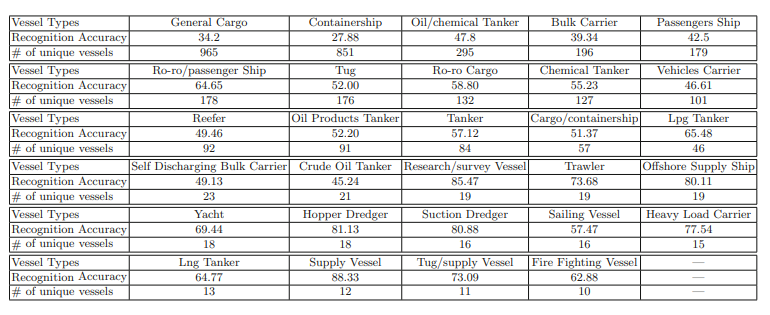
\includegraphics[width=\textwidth,height=10cm,keepaspectratio=true]{src/Images/marvel_accuracy.PNG}
    \caption{
     Breakdown of recognition accuracies across the 29 vessel types\cite{gundogdu2017marvel}. 
     }
\end{figure}
\\

In the previous two papers, the authors discussed two important tasks in the maritime computer vision domain, namely vessel and maritime environment Image Segmentation and vessel-level Image Classification. In contrast, the following paper introduces a new dataset designed specifically for Object Detection in maritime applications. The paper, authored by Soloviev et al. and titled "COMPARING CNN-BASED OBJECT DETECTORS ON TWO NOVEL MARITIME DATASETS,"\cite{soloviev2020comparing} describes the collection of two datasets, collected in the Finnish Archipelago, consisting of various maritime vessels performing different tasks, under different weather and lighting conditions. The authors then benchmarked the dataset using three of the most popular and widely available state-of-the-art CNN-based object detection algorithms. They reported the accuracy and average throughput (measured in frames per second) of each model. 
\\

The authors of the study created two datasets for their research. They sourced the images for the first dataset using a video camera with a 65° field of view mounted on a sightseeing watercraft. The collection comprised over 135 videos captured during daytime conditions over a period of 13 days while the watercraft traveled between Turku and Ruissalo cities in South West Finland, along the Aura River and into the Finnish archipelago. The weather conditions varied between sunny and cloudy, with instances of fog and rain. The environment consisted mainly of urban landscapes. To evaluate the object detection models, the authors extracted 4800 photos from the videos and after eliminating redundancy, they selected 400 photos and annotated them precisely. Dataset one contained 850 annotated vessels.
\\

For dataset two, the authors focused on adding diversity to the data and captured images of the open-sea environment. They used an alternative sensing solution consisting of RGB (visible spectrum) and IR (thermal) cameras. The cameras were synced with each other, and their outputs were stitched together to form panoramic images. The images were sampled one frame per second and all vehicles, such as passenger vessels, motorboats, sailboats, or docked vessels within each IR/RGB sequence were manually annotated with a bounding box. Dataset two had 1,750 images captured using visible cameras and contained 9,137 vessel objects.
\\

For dataset evaluation, the authors trained both one-stage (SSD) and two-stage (Faster R-CNN and R-FCN) object detectors. The models were pre-trained using the MS COCO object detection dataset. The training dataset includes 3,146 images. As part of their work, the authors also researched the impact of different model backbones/feature extractors to find the backbone with best performance with respect to runtime and accuracy. For this task, the authors collected model inference on the test dataset using an SSD with different feature extractors. The backbones explored were MobileNet-v1, MobileNet-v2, and Inception-v2. Furthermore, the authors evaluated other detectors using three different feature extractors such as NasNet, ResNet50, ResNet101, and
Inception-resnet-v2. Combining these feature extractors
with the three proposed object detectors, a total of nine methods were investigated. For both datasets, the highest AP achieved was by faster R-CNN using the ResNet101 backbone. 
\begin{figure}[H]
    \centering
    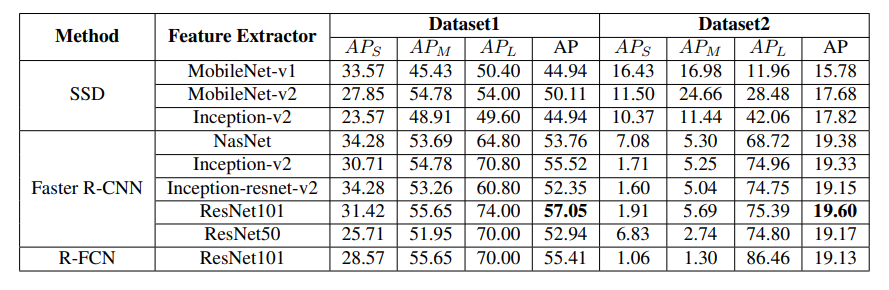
\includegraphics[width=\textwidth,height=10cm,keepaspectratio=true]{src/Images/solv_results.PNG}
    \caption{
     Results from the author's experiments\cite{soloviev2020comparing}. AP(Small), AP(Medium), AP(Large) and AP(all) represent the AP for small, medium, and large objects.\cite{soloviev2020comparing}
     }
\end{figure}
\\

The authors of the study also found that the size of objects had a significant impact on the performance of the detection models, especially when it comes to smaller objects. To confirm this, the authors classified all annotated objects in both datasets into three categories: small, medium, and large, based on the definition of the COCO challenge. The authors found that the datasets contained more small and medium-sized objects than large objects. According to the experiments, the accuracy of the detection decreased significantly with a decrease in object size. The best-performing method (Faster R-CNN with ResNet101) showed a decrease of almost 42.58\% and 73.48\% in the average precision (AP) from large to small objects on Dataset1 and Dataset2, respectively. Among the various SSD configurations tested, the MobileNet-v2 backbone was found to be the most accurate for detecting medium and large objects in both datasets. However, SSD with MobileNet-v1 achieved higher accuracy for small objects. Overall, the best result for both datasets for all objects was generated by Faster R-CNN with ResNet101.
\begin{figure}[H]
    \centering
    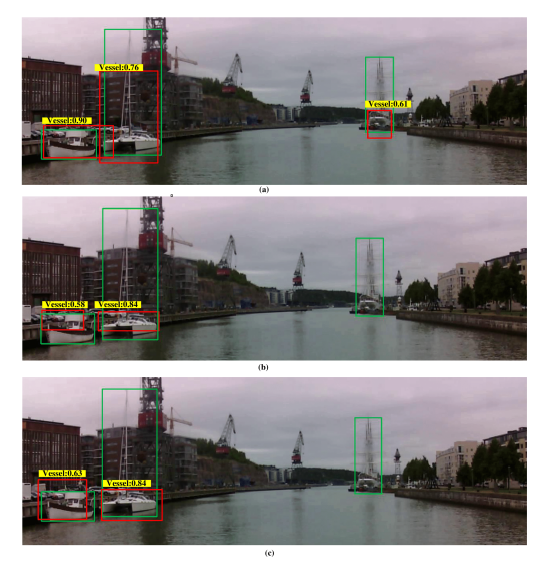
\includegraphics[width=\textwidth,height=10cm,keepaspectratio=true]{src/Images/solv_res_1.PNG}
    \caption{
     Detection results for Dataset 1 using different models: (a) SSD, (b) Faster R-CNN, and (c) R-FCN. The ground truth bounding boxes are represented by green, while the predicted boxes are colored red. Each output box is associated with a category label and a confidence score between 0 to 1. (0\% to 100\%)\cite{soloviev2020comparing}
     }
\end{figure}
\\

Regarding the run time, the authors compared the selected models using the same hardware platform. All selected detectors were tested on an example image of resolution 1200×400 pixels from the dataset. The inference platform consisted of 4x NVIDIA Tesla P100 GPUs connected in pairs. The experiments showed that Faster R-CNN with Inception-resnetv2 had the least running time (1.04 seconds) but was 4.7\% less accurate than the best-performing Faster R-CNN model with ResNet101 backbone. 
\begin{figure}[H]
    \centering
    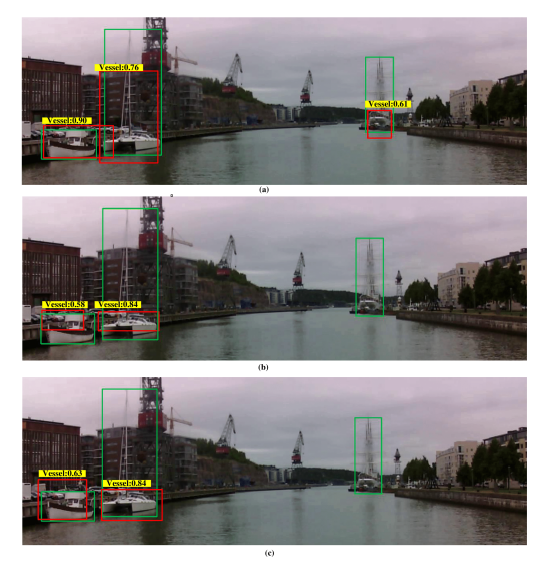
\includegraphics[width=\textwidth,height=10cm,keepaspectratio=true]{src/Images/solv_res_1.PNG}
    \caption{
     Detection results for Dataset 2 using different models: (a) SSD, (b) Faster R-CNN, and (c) R-FCN. The ground truth bounding boxes are represented by green, while the predicted boxes are colored red. Each output box is associated with a category label and a confidence score between 0 to 1. (0\% to 100\%)\cite{soloviev2020comparing}
     }
\end{figure}
\\

One of the biggest challenges facing marine perception researchers is the limited availability of training data, due to the difficulties associated with capturing data for this task. These challenges include acquiring a vessel, finding the right environmental conditions, and having limited dataset diversity. For deep learning methods to be successful and applicable in real-time applications, they require a large amount of data. To tackle the challenge of the lack of diverse data in the marine space, the authors of "Ship Classification Using Deep Learning Techniques for Maritime Target Tracking" by Leclerc et al\cite{leclerc2018ship} have used the Transfer Learning approach to train CNN models. This approach involves reusing a network previously trained on a large dataset, such as imagenet, and reusing/freezing the layers of the network used for developing the feature pyramid. Only the last fully connected layer is modified with another fully connected layer, which is then trained using the limited amount of data that's available. Transfer learning also provides an additional benefit of preventing over-fitting by using a large number of images and a large number of classes to train the model initially. The authors used the classification labels in improving the current hidden Markov models based object tracking estimation algorithms. 
\begin{figure}[H]
    \centering
    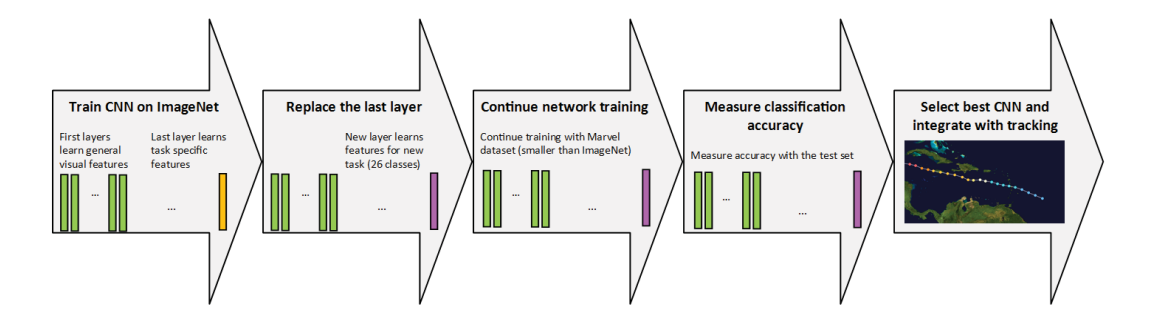
\includegraphics[width=\textwidth,height=10cm,keepaspectratio=true]{src/Images/leclerc_approach.PNG}
    \caption{The author's approach for applying transfer learning to the ship classification and tracking problem.\cite{leclerc2018ship}
     }
\end{figure}
\\

The authors evaluated three pre-trained CNN architectures - AlexNet, ResNet, and Inception - with different depths or numbers of hidden layers. They pre-trained the network using the ImageNet dataset. The layers of this network, until the last fully connected layer, are effective in developing features for general image classification. The initial CNN layers respond to various oriented edges and lines in the image, while the middle layers react to parts of an object, such as corners and surface boundaries. In contrast, higher layers react to larger object parts and even complete objects. Therefore, the last layers of these neural networks tend to be more specific to the datasets and tasks performed. To achieve transfer learning, the authors replaced these layers with layers trained more specifically on their dataset. The authors selected the MARVEL dataset, which contains around 140,000 labeled visible images of ships extracted from 2,000,000 images. The pre-trained networks were trained on the imagenet dataset. The authors tested various model architectures, including AlexNet, ResNets, Inceptionv1, and Inception-v3. The authors also test various regularization values to achieve the best balance between model complexity and validation accuracy. As part of their work, the authors also tried to improve tracking algorithms using classification results. The authors used the marvel dataset using the Stat5 taxonomy to fine-tune the networks. 

\begin{figure}[H]
    \centering
    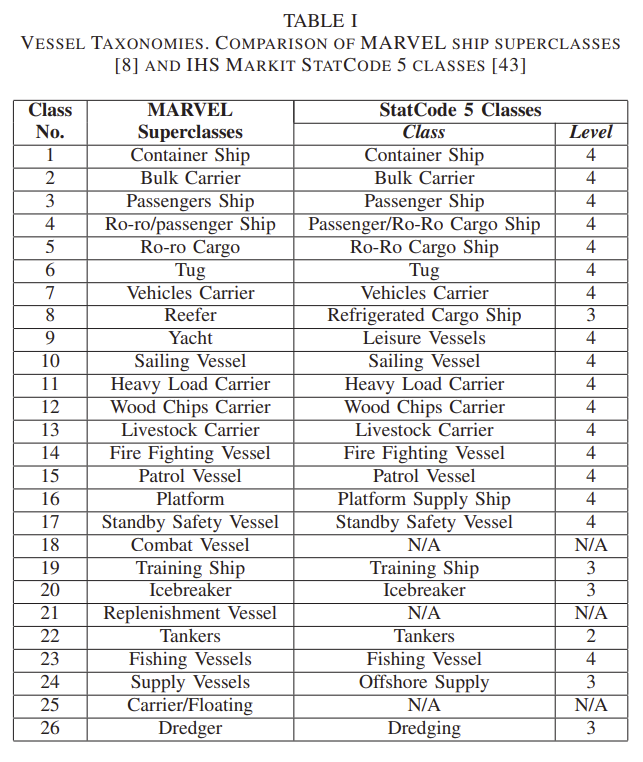
\includegraphics[width=\textwidth,height=10cm,keepaspectratio=true]{src/Images/stat5_taxonomy.png}
    \caption{How marvel dataset classes are converted to their stat5 equivalent\cite{leclerc2018ship}
     }
\end{figure}
\\

The author's results are shown in Figure 2.24 below. The best score obtained was
78.73\% accuracy. For the best learning rate, the authors used a rotational learning rate based on the epoch and found the best regularization value of 0.0005. Out of the compared models, Inception-v3 performed better than both ResNets and AlexNet for maritime vessel classification. ResNets, with 34 layer architecture, obtained the best accuracy. For the Inception architecture, inception v3 performed the best overall. 
\begin{figure}[H]
    \centering
    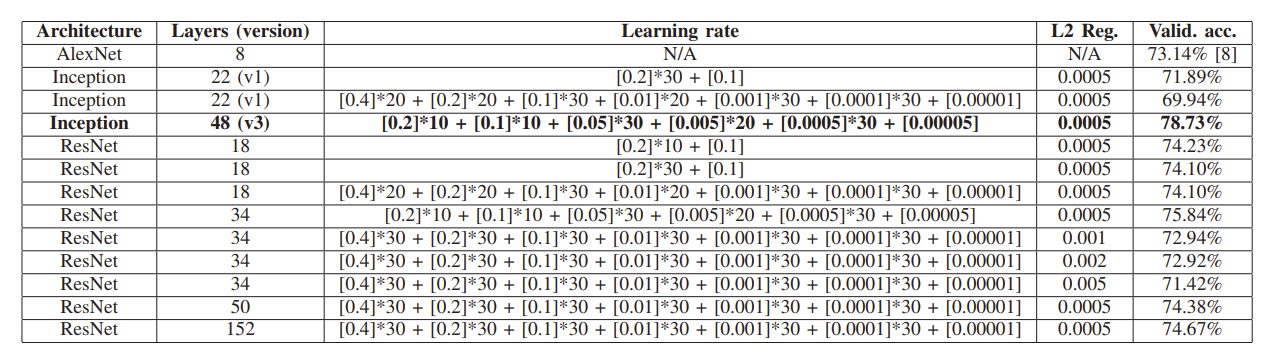
\includegraphics[width=\textwidth,height=10cm,keepaspectratio=true]{src/Images/leclerc_res.png}
    \caption{Performance of the various networks finetuned by the authors. \cite{leclerc2018ship}
     }
\end{figure}
\\